%!TEX encoding = UTF-8 Unicode
%!TEX root = ../lect-w04.tex

\ifkompendium\else
\begin{SlideExtra}{Denna vecka: Objekt}
\begin{itemize}
\item Övning \texttt{objects} innehåller bland annat:
\begin{itemize}
\item hur man kan kapsla in funktioner och variabler i singelobjekt (kallas även moduler)
\item hur man kan skapa namnrymder, hantera namnöverskuggning, och använda punktnotation
%\item skapa objekt med hjälp av tupler
%\item lat initialisering
%\item jar-fil, paket, namnbyte vid import
\item använda färdiga klasser, t.ex. \code{java.awt.Color}
\item händelsehantering i ett grafiskt fönster
\end{itemize}

\item På laboration \texttt{blockmole} lär du dig bland annat:
\begin{itemize}
  \item att dela upp din kod i flera singelobjekt
  \item att använda färdig klass i jar-fil: \code{introprog.PixelWindow}
  \item att skapa ett större program i form av ett grafiskt spel
  \item sätta samman det vi lärt hittills om uttryck, program och funktioner
\end{itemize}

\item Senaste versionen av kursbiblioteket \code{introprog} är $1.1.4$ och jar-filens namn är \code{introprog_2.12-1.1.4.jar} \\Se dokumentation här: \url{http://cs.lth.se/pgk/api}
\end{itemize}
\end{SlideExtra}
\fi


\Subsection{Vad är ett objekt?}



\begin{Slide}{Vad rymmer sköldpaddan i Kojo i sitt tillstånd?}
\centering
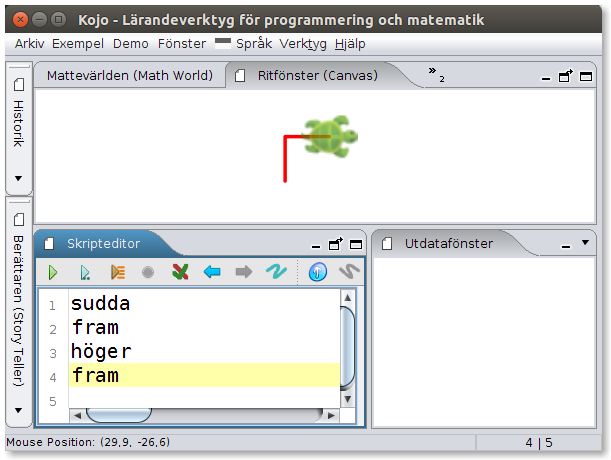
\includegraphics[width=0.7\textwidth]{../img/kojo}

\pause position, riktning, färg, bredd, penna uppe/nere, fyll-färg
\end{Slide}



\begin{Slide}{Vad är ett objekt?}
\begin{itemize}
\item Ett objekt är en abstraktion som...
\begin{itemize}
  \item kan innehålla \Emph{data} som objektet ''håller reda på'' och
  \item kan erbjuda \Emph{operationer} som \emph{gör} något eller ger ett \emph{värde}
\end{itemize}

\pause

\item Exempel: Sköldpaddan i Kojo 
\includegraphics[width=0.08\textwidth]{../img/turtle.png}
\begin{itemize}
  \item Vilken \Emph{data} sparas av sköldpaddan?
  \pause
  \item[] position, rikting, pennfärg, ...

  \item Vilka \Emph{operationer} kan man be sköldpaddan att utföra?

  \item[] fram, höger, vänster, ...
  \pause


\end{itemize}

\item Terminologi:
\begin{itemize}
  \item objektets data sparas i variabler som kallas \Alert{attribut}
  \item alla variabelvärden utgör tillsammans objektets \Alert{tillstånd}
  \item operationerna är funktioner i objektet och kallas \Alert{metoder}
  \item attribut, metoder (och annat i objektet) kallas \Alert{medlemmar}
\end{itemize}
\end{itemize}
\end{Slide}



\begin{Slide}{Deklarera, allokera, referera}
Olika saker man kan göra med objekt:
\begin{itemize}
  \item \Emph{deklarera}: att skriva kod som beskriver objekt; \\
  finns flera sätt: singelobjekt, klass, tupel, ...
  \item \Emph{allokera}: att skapa plats i minnet för objektet vid körtid
  \item \Emph{referera}: att använda objektet via ett namn;\\
  man kommer åt innehållet i ett objekt med \Alert{punktnotation}: \\
  \code{ref.medlem}
  \pause
  \item (\Emph{avallokera}): att frigöra minne för objekt som inte längre används;
  detta \Alert{sker automatiskt} i Scala och Java, men i många andra språk,
  t.ex. C++, får man själv hålla reda på avallokering,
  vilket är knepigt och det blir lätt svåra buggar.
\end{itemize}
\end{Slide}


\begin{Slide}{Allokera objekt}\SlideFontSmall
Det finns flera olika sätt att skapa objekt:
\begin{itemize}

\item Använda en \Emph{färdig funktion} som skapar ett objekt åt oss, t.ex. \code{apply}:
\begin{Code}
Vector(1,2,3)  // skapa Vector-objekt med apply-metod
Vector.apply(1,2,3)  // explicit apply
\end{Code}
{\SlideFontSmall En funktion som skapar objekt kallas \Alert{fabriksmetod}.\vspace{0.5em}}

\item Använda \code{new} (mer om detta senare: då behövs en klass):
\begin{Code}
new introprog.PixelWindow(title = "Hej!") // skapa fönsterobjekt
\end{Code}
{\SlideFontSmall Med \code{new} kan man skapa \Alert{många upplagor} av samma typ av objekt.\vspace{0.5em}}

\item Deklarera ett \Emph{singelobjekt} med nyckelordet \code{object}
\begin{itemize}\SlideFontSmall
  \item Ett singelobjekt finns i exakt \Alert{en} upplaga.
  \item Det allokeras \Alert{automatiskt} första gången man refererar objektet; \\
  man behöver inte, och kan inte, skriva \code{new}.
  \pause
  \item Medlemmar i ett Scala-singelobjekt liknar \jcode{static}-medlemmar i en Java/C++/C\#-klass.
\end{itemize}
\item Använda en \Emph{tupel}, exempel: \code{val p = (200, 300)}
\end{itemize}
\end{Slide}

\Subsection{Singelobjekt}

\begin{Slide}{Vad är ett singelobjekt?}
\begin{itemize}
\item Ett singelobjekt \Eng{singelton} deklareras med nyckelordet \code{object} och kan användas för att samla \Emph{medlemmar} \Eng{members} som \Alert{hör ihop}.
\item Kallas också \Emph{modul}.
\item Medlemmarna kan t.ex. vara \Emph{variabler} (\code{val}, \code{var}) och \Emph{metoder} (\code{def}). En \Alert{metod} är en \Emph{funktion} i ett objekt.
\item Exempel: singelobjekt/modul som hanterar highscore:
\begin{Code}
object Highscore {
  var highscore = 0
  def isHighscore(points: Int): Boolean = points > highscore
}
\end{Code}
\end{itemize}
\pause
{\SlideFontSmall Tanken är ofta att abstraktionen ska vara användbar i annan kod, för att underlätta när man bygger applikationer, och kallas då även ett API (Application Programming Interface). Exempel: ett highscore-API}
\end{Slide}


\begin{Slide}{Allokering: minne reserveras med plats för data}
\begin{Code}
object Highscore {
  var highscore = 0
  def isHighscore(points: Int): Boolean = points > highscore
}
\end{Code}
\pause
\begin{tikzpicture}[font=\large\sffamily]
\matrix [matrix of nodes, row sep=0, column 2/.style={nodes={rectangle,draw,minimum width=0.8cm}}] (mat)
{
\texttt{HighScore}   &  \makebox(10,10){ }\\
%\texttt{g2}   &  \makebox(16,12){ }\\
};
\node[cloud, cloud puffs=13.0, cloud ignores aspect, minimum width=2cm, minimum height=3.8cm,
 align=center, draw] (x) at (5.8cm, -1.5cm) {
 \begin{tabular}{r l}
 \texttt{highscore} & \fbox{~~~~~0~~} \\

 \end{tabular}
 };
\filldraw[black] (1.2cm,0.0cm) circle (3pt) node[] (ref) {};
 \draw [arrow, line width=0.7mm] (ref) -- (x);
% \node[cloud, cloud puffs=15.7, cloud ignores aspect, %minimum width=5cm, minimum height=2cm,
% align=center, draw] (g2) at (5cm, -2cm) {Gurka-\\objekt};
% \filldraw[black] (0.4cm,-0.4cm) circle (3pt) node[] (g2ref) {};
% \draw [arrow] (g2ref) -- (g2);
\end{tikzpicture}
\end{Slide}


\begin{Slide}{Punktnotation, tillståndsförändring med tilldelning}
\begin{REPLnonum}
scala> Highscore.isHighscore(5)
res0: Boolean = true

scala> Highscore.highscore = 42
\end{REPLnonum}
\pause
\begin{tikzpicture}[font=\large\sffamily]
\matrix [matrix of nodes, row sep=0, column 2/.style={nodes={rectangle,draw,minimum width=0.8cm}}] (mat)
{
\texttt{HighScore}   &  \makebox(10,10){ }\\
%\texttt{g2}   &  \makebox(16,12){ }\\
};
\node[cloud, cloud puffs=13.0, cloud ignores aspect, minimum width=2cm, minimum height=3.8cm,
 align=center, draw] (x) at (5.8cm, -1.5cm) {
 \begin{tabular}{r l}
 \texttt{highscore} & \fbox{~~~~42~~} \\

 \end{tabular}
 };
\filldraw[black] (1.2cm,0.0cm) circle (3pt) node[] (ref) {};
 \draw [arrow, line width=0.7mm] (ref) -- (x);
% \node[cloud, cloud puffs=15.7, cloud ignores aspect, %minimum width=5cm, minimum height=2cm,
% align=center, draw] (g2) at (5cm, -2cm) {Gurka-\\objekt};
% \filldraw[black] (0.4cm,-0.4cm) circle (3pt) node[] (g2ref) {};
% \draw [arrow] (g2ref) -- (g2);
\end{tikzpicture}
\end{Slide}


\begin{Slide}{Punktnotation och operatornotation}
Punktnotation på formen\\~\\
\code{objekt.metod(argument)}
\\~\\kan även skrivas med \Emph{operatornotation}:\\~\\
\code{objekt metod argument}
\\~\\Exempel:\\
\code{1 + 2}\\
\code{Highscore isHighscore 1000}

\end{Slide}


\begin{Slide}{Namnrymd och skuggning}
\begin{itemize}\SlideFontSmall
  \item En \Emph{namnrymd}\footnote{\url{https://sv.wikipedia.org/wiki/Namnrymd}}  \Eng{name space} är en omgivning (kontext) i vilken alla namn är unika. Genom att skapa flera olika namnrymder
  kan man undvika ''\Alert{krockar}'' mellan lika namn med olika betydelser (homonymer). \\
  Exempel: mejladresser \code{kim@företag1.se}  ~$\neq$~  \code{kim@företag2.se}
  \item Medlemmarna i ett singelobjekt finns i en egen namnrymd,
  där alla namn måste vara unika. De ''krockar'' inte med namn ''utanför'' objektet. Dock kan det förekomma \Alert{skuggning} \Eng{shadowing}:
\end{itemize}
\begin{Code}
object Game {

  val highscore = 42   // ett annat värde än Game.Highscore.highscore

  object Highscore {
    var highscore = 0  // ett annat värde än Game.highscore
    def isHighscore(points: Int): Boolean = points > highscore
  }
}
\end{Code}

\end{Slide}



\begin{Slide}{Inkapsling: att dölja interna delar}\SlideFontSmall
Med nyckelordet \code{private} döljs interna delar för omvärlden.
Privata medlemmar kan bara refereras \emph{inifrån} objektet.
Denna princip kallas \Emph{inkapsling} \Eng{encapsulation}.
\begin{CodeSmall}
object Highscore {
  private var myHighscore = 0        // namnet myHighscore syns ej utåt
  def highscore: Int = myHighscore   // en s.k. getter ger ett attributvärde
  def isHighscore(points: Int): Boolean = points > myHighscore
  def update(points: Int): Unit = if (isHighscore(points)) myHighscore = points
}
\end{CodeSmall}
\pause
Varför har man nytta av detta?
\begin{itemize}
  \item Förhindra att man av misstag ändrar objekts tillstånd på fel sätt.
  \item Förhindra användning av kod som i framtiden kan komma att ändras.
  \item Erbjuder en enklare ''utsida'' genom dölja komplexitet ''på insidan''.
  \item Inte ''skräpa ner'' namnrymden med ''onödiga'' namn.
\end{itemize}
Nackdelar:
\begin{itemize}
  \item Begränsar användningen, har ej tillgång till alla delar.
  \item Svårare att experimentera med ett API medan man försöker förstå det.
\end{itemize}
\end{Slide}



\begin{Slide}{Idiom: Privata variabler med understreck vid ''krock''}\SlideFontSmall
\Emph{Idiom}: (d.v.s. ett typiskt, allmänt accepterat sätt att skriva kod)
\begin{itemize}
  \item Om namnet på en privat variabel krockar med namnet på en getter
  brukar man börja det privata namnet med ett understreck:
\end{itemize}

\begin{CodeSmall}
object Highscore {
  private var _highscore = 0
  def highscore: Int = _highscore
  def isHighscore(points: Int): Boolean = points > _highscore
  def update(points: Int): Unit = if (isHighscore(points)) _highscore = points
}
\end{CodeSmall}

\pause

(Detta problem uppkommer inte i Java m.fl. språk, där metoder och attribut finns i \emph{olika} namnrymder.
Men i Scala har man valt att principen om \Emph{enhetlig access} ska gälla; alla medlemmar finns därmed i en gemensam namnrymd.)

\end{Slide}


\begin{Slide}{Modul}

\begin{itemize}
  \item En modul samlar kod som utgör en sammanhållen, avgränsad \Emph{uppsättning abstraktioner} som kan användas av annan kod  för att lösa ett specifikt (del)problem.
  \item I Scala finns två sätt att skapa moduler:\footnote{\href{https://en.wikipedia.org/wiki/Modular_programming}{en.wikipedia.org/wiki/Modular\_programming}}
  \begin{itemize}
    \item \Emph{singelobjekt} med nyckelordet \code{object} och
    \item \Emph{paket} med nyckelordet \code{package}
    \pause
    \item Liknar varandra; t.ex. kan man använda punktnotation och göra \code{import} på medlemmar i både singelobjekt och paket.
    \pause
    \item Skillnader:
    \begin{itemize}
      \item paket medför att \Alert{underkataloger} för maskinkoden skapas vid kompilering
      \item paket innehåller inte variabler på topp-nivå; dessa behöver ligga inuti singelobjekt eller klasser
    \end{itemize}
    \item (I Scala kan man kombinera begreppen: \code{package object})
  \end{itemize}

\end{itemize}
\end{Slide}





\begin{Slide}{Exempel: singelobjektet med tillstånd} \SlideFontSmall
\begin{Code}[basicstyle=\ttfamily\fontsize{9}{11}\selectfont]
object mittBankkonto {
  val kontonr: Long        = 1234567L
  var saldo: Int           = 1000
  def ärSkuldsatt: Boolean = saldo < 0
}
\end{Code}
\begin{REPLnonum}
scala> mittBankkonto.saldo -= 25000

scala> mittBankkonto.ärSkuldsatt
res0: Boolean = true
\end{REPLnonum}

(Vi ska i nästa vecka se hur man med s.k. klasser kan skapa många upplagor av samma  typ av objekt, så att vi kan ha flera olika bankkonto.)
\end{Slide}



\begin{Slide}{Exempel: tillstånd, attribut}
Ett objekts \Emph{tillstånd} är den samlade uppsättningen av värden av alla de attribut som finns i objektet.
\begin{Code}[basicstyle=\ttfamily\fontsize{9}{11}\selectfont]
object mittBankkonto {
  val kontonr: Long        = 1234567L
  var saldo: Int           = 1000
  def ärSkuldsatt: Boolean = saldo < 0
}
\end{Code}
\begin{tikzpicture}[font=\large\sffamily]
\matrix [matrix of nodes, row sep=0, column 2/.style={nodes={rectangle,draw,minimum width=0.8cm}}] (mat)
{
\texttt{mittBankkonto}   &  \makebox(10,10){ }\\
%\texttt{g2}   &  \makebox(16,12){ }\\
};
\node[cloud, cloud puffs=13.0, cloud ignores aspect, minimum width=2cm, minimum height=3.8cm,
 align=center, draw] (x) at (5.8cm, -1.5cm) {
 \begin{tabular}{r l}
 \texttt{kontonr} & \fbox{1234567L} \\
 \texttt{saldo} & \fbox{1000}\\
 \end{tabular}
 };
\filldraw[black] (1.7cm,0.0cm) circle (3pt) node[] (ref) {};
 \draw [arrow, line width=0.7mm] (ref) -- (x);
% \node[cloud, cloud puffs=15.7, cloud ignores aspect, %minimum width=5cm, minimum height=2cm,
% align=center, draw] (g2) at (5cm, -2cm) {Gurka-\\objekt};
% \filldraw[black] (0.4cm,-0.4cm) circle (3pt) node[] (g2ref) {};
% \draw [arrow] (g2ref) -- (g2);
\end{tikzpicture}
\end{Slide}


\begin{Slide}{Tillståndsändring}

När en variabel tilldelas ett nytt värde sker en \Emph{tillståndsändring}. Ett \Emph{förändringsbart objekt} \Eng{mutable object} har ett \Emph{förändringsbart tillstånd} \Eng{mutable state}.

\begin{REPLnonum}
scala> mittBankkonto.saldo -= 25000

scala> mittBankkonto.saldo
res1: Int = -24000
\end{REPLnonum}
\begin{tikzpicture}[font=\large\sffamily]
\matrix [matrix of nodes, row sep=0, column 2/.style={nodes={rectangle,draw,minimum width=0.8cm}}] (mat)
{
\texttt{mittBankkonto}   &  \makebox(10,10){ }\\
%\texttt{g2}   &  \makebox(16,12){ }\\
};
\node[cloud, cloud puffs=13.0, cloud ignores aspect, minimum width=2cm, minimum height=3.8cm,
 align=center, draw] (x) at (5.8cm, -1.5cm) {
 \begin{tabular}{r l}
 \texttt{kontonr} & \fbox{1234567L} \\
 \texttt{saldo} & \fbox{-24000}\\
 \end{tabular}
 };
\filldraw[black] (1.7cm,0.0cm) circle (3pt) node[] (ref) {};
 \draw [arrow, line width=0.7mm] (ref) -- (x);
% \node[cloud, cloud puffs=15.7, cloud ignores aspect, %minimum width=5cm, minimum height=2cm,
% align=center, draw] (g2) at (5cm, -2cm) {Gurka-\\objekt};
% \filldraw[black] (0.4cm,-0.4cm) circle (3pt) node[] (g2ref) {};
% \draw [arrow] (g2ref) -- (g2);
\end{tikzpicture}
\end{Slide}

\Subsection{Paket}


\begin{Slide}{Deklarera paket}
Med nyckelordet \code{package} först i en kodfil ges alla deklarationer en gemensam namnrymd.\\
\vspace{1em}
Denna kod ligger i filen f1.scala:
\begin{Code}
package mittpaket

object A {
  def main(args: Array[String]) : Unit = B.hej
}
\end{Code}

Denna kod ligger i filen f2.scala:
\begin{Code}
package mittpaket

object B {
  def hej = println("hej mittpaket")
}
\end{Code}
Singelobjekten \code{A} och \code{B} finns båda i namnrymden \code{mittpaket}.
\end{Slide}

\begin{Slide}{Kompilera paket}\SlideFontSmall
Paketdeklarationer medför att kompilatorn placerar bytekodfiler i en katalog med samma namn som paketet:
\begin{REPL}
> scalac f1.scala f2.scala     // samkompilering av två filer
> ls
f1.scala  f2.scala  mittpaket
> ls mittpaket
A.class  A$.class  B.class  B$.class
> scala mittpaket.A
hej mittpaket
\end{REPL}
\pause
Idiom, syntax och semantik:
\begin{itemize}
  \item Paketnamn brukar bestå av enbart små bokstäver.
  \item Om paketnamn innehåller punkt(er), skapas nästlade underpaket, exempel:  \code{p1.p2.p3} kompilerar kod till katalogen \code{p1/p2/p3}
  \item Det är ovanligt, men man kan i Scala ha flera paket och även nästlade paket i \Alert{samma} kodfil
  om man använder klammerparenteser, exempel:\\
  \code|package p1 { object A; package p2 { object B }}|
\end{itemize}
\end{Slide}

\begin{Slide}{Paket i REPL}
Paket funkar inte i REPL direkt; använd \code{:paste -raw}

\begin{REPLnonum}
scala> package mittpaket { object X { def hej = println("Hej") } }
<console>:1: error: illegal start of definition
       package mittpaket { object X { def hej = println("Hej") } }
       ^

scala> :paste -raw
// Entering paste mode (ctrl-D to finish)

package mittpaket { object X { def hej = println("Hej") } }

// Exiting paste mode, now interpreting.


scala> mittpaket.X.hej
Hej

\end{REPLnonum}

\end{Slide}


\Subsection{Tupler}


\begin{Slide}{Vad är en tupel?}\SlideFontSmall

\begin{itemize}
\item En $n$-tupel är ett objekt som samlar $n$ st objekt i en enkel datastruktur med koncis syntax;
du behöver bara parenteser och kommatecken för att skapa tupel-objekt: ~~\code{(1,'a',"hej")}
\item Elementen kan alltså vara av \Alert{olika} typ.

\item
\code{(1,'a',"hej")} är en \Emph{3-tupel} av typen: \code{(Int, Char, String)}

\pause

\item Du kan komma åt de enskilda elementen med \Emph{\code{_1}}, \Emph{\code{_2}}, ...  \code{_}$n$

\begin{REPL}
scala> val t = ("hej", 42, math.Pi)
t: (String, Int, Double) = (hej,42,3.141592653589793)

scala> t._1
res0: String = hej

scala> t._2
res1: Int = 42
\end{REPL}

\pause

\item Tupler är praktiska när man inte vill ta det lite större arbetet att skapa en egen klass.
(Men med klasser kan man göra mycket mer än med tupler.)

\item I Scala 2.12 kan du skapa tupler upp till en storlek av 22 element.
\\ (Behöver du fler element, använd i stället en samling, t.ex. \code{Vector}.)

\end{itemize}

\end{Slide}


\begin{Slide}{Tupler som parametrar och returvärde.}\SlideFontSmall

\begin{itemize}

\item Tupler är smidiga som \Emph{parametrar} om man vill kombinera värden som hör ihop, till exempel
 x- och y-värdena i en punkt: \code{(3, 4)}
\pause
\item Tupler är smidiga när man på ett enkelt och typsäkert sätt
vill låta en funktion \Emph{returnera mer än ett värde}.

\begin{REPL}
scala> def längd(p: (Double, Double)): Double = math.hypot(p._1, p._2)

scala> def vinkel(p: (Double, Double)): Double = math.atan2(p._1, p._2)

scala> def polär(p: (Double, Double)) = (längd(p), vinkel(p))

scala> polär((3,4))
res2: (Double, Double) = (5.0,0.6435011087932844)

\end{REPL}
\vspace{0.5em}
\item Om typerna passar kan man skippa dubbla parenteser vid \Emph{ensamt tupel-argument}:
\begin{REPL}
scala> polär(3,4)
res3: (Double, Double) = (5.0,0.6435011087932844)
\end{REPL}
\item[] {\SlideFontTiny\href{https://sv.wikipedia.org/wiki/Pol\%C3\%A4ra_koordinater}{https://sv.wikipedia.org/wiki/Polära\_koordinater}}


\end{itemize}
\end{Slide}



\begin{Slide}{Ett smidigt sätt att skapa 2-tupler med metoden \texttt{->}}
Det finns en metod vid namn \code{->} som kan användas på objekt av \Alert{godtycklig} typ för att \Emph{skapa par}:

\vspace{0.8em}
\begin{REPL}
scala> ("Ålder", 42)
res0: (String, Int) = (Ålder,42)

scala> "Ålder".->(42)
res1: (String, Int) = (Ålder,42)

scala> "Ålder" -> 42
res2: (String, Int) = (Ålder,42)

scala> Vector("Ålder" -> 42, "Längd" -> 178, "Vikt" -> 65)
res3: scala.collection.immutable.Vector[(String, Int)] =
        Vector((Ålder,42), (Längd,178), (Vikt,65))


\end{REPL}
\end{Slide}




\Subsection{Fördröjd initialisering}

\begin{Slide}{Lata variabler och fördröjd initialisering}
Med nyckelordet \code{lazy} före \code{val} sker ''\Emph{lat}'' evaluering av initialiseringsuttrycket. Motsatsen (det normala i Scala) kallas \Alert{strikt} evaluering.
\begin{REPL}
scala> val strikt = Vector.fill(1000000)(math.random)
strikt: scala.collection.immutable.Vector[Double] =
 Vector(0.7583305221813246, 0.9016192590993339, 0.770022134260162, 0.15667718184929746, ...

scala> lazy val lat = Vector.fill(1000000)(math.random)
lat: scala.collection.immutable.Vector[Double] = <lazy>

scala> lat
res0: scala.collection.immutable.Vector[Double] =
  Vector(0.5391685014341797, 0.14759775960530275, 0.722606095900537, 0.9025572787055386, ...
\end{REPL}

En \code {lazy val} initialiseras \Alert{inte} vid deklarationen utan när den \Alert{refereras första gången}. Uttrycket som anges i deklarationen evalueras med s.k. \Emph{fördröjd evaluering} (även ''lat'' evaluering).
\end{Slide}




\begin{Slide}{Singelobjekt är lata}

\begin{itemize}
  \item Singelobjekt allokeras \Alert{inte} direkt vid deklaration; allokeringen sker först då objektet refereras första gången.

\pause

  \item Exempel:

\end{itemize}

\begin{Code}
object mittLataObjekt {
  println("jag är lat")
  val storArray = { println("skapar stor Array"); Array.fill(10000)(42) }
  lazy val ännuStörreArray = Array.fill(Int.MaxValue)(42)
}
\end{Code}

När sker utskrifterna?

När allokeras variablerna?

\end{Slide}




\begin{Slide}{Vad är skillnaden mellan \texttt{val}, \texttt{var}, \texttt{def} och \texttt{lazy val}?}
\begin{Code}[basicstyle=\ttfamily\fontsize{8}{11}\selectfont]
object exempel {
  println("hej exempel")
  val förAlltidSammaReferens  = { println("hej val"); math.random }
  var kanÄndrasMedTilldelning = { println("hej var"); math.random }
  def evaluerasVidVarjeAnrop  = { println("hej def"); math.random }
  lazy val fördröjdInit  = { println("hej lazy val"); math.random }
}
\end{Code}
\vspace{1em}\pause
Lat evaluering är en viktig princip inom funktionsprogrammering som möjliggör effektiva, oföränderliga datastrukturer där element allokeras först när de behövs. \\
\href{https://en.wikipedia.org/wiki/Lazy_evaluation}{en.wikipedia.org/wiki/Lazy\_evaluation}
\end{Slide}




\Subsection{Funktioner är objekt}

\begin{Slide}{Programmeringsparadigm}
\href{https://en.wikipedia.org/wiki/Programming_paradigm}{en.wikipedia.org/wiki/Programming\_paradigm}:
\begin{itemize}
\item \Emph{Imperativ programmering}: programmet är uppbyggt av sekvenser av olika satser som läser och \Alert{ändrar} tillstånd
\item \Emph{Objektorienterad programmering}: en sorts imperativ programmering där programmet består av objekt som kapslar in tillstånd och erbjuder operationer som läser och \Alert{ändrar} tillstånd.
\item \Emph{Funktionsprogrammering}: programmet är uppbyggt av samverkande (äkta) funktioner som \Alert{undviker} föränderlig data och tillståndsändringar. Oföränderliga datastrukturer skapar effektiva program i kombination med lat evaluering och rekursion.
\end{itemize}
\end{Slide}


\begin{Slide}{Funktioner är äkta objekt i Scala}
Scala visar hur man kan \Alert{förena} \Eng{unify} \\ \Emph{objektorientering} och \Emph{funktionsprogrammering}: \\\vspace{0.5em}

\textbf{En funktion är ett objekt som har en \code{apply}-metod.}
\pause
\begin{REPLnonum}
scala> object öka {
         def apply(x: Int) = x + 1
       }

scala> öka.apply(1)
res0: Int = 2

scala> öka(1)   // metoden apply behöver ej skrivas explicit
res1: Int = 2
\end{REPLnonum}
\end{Slide}



\begin{Slide}{Fördjupning: Äkta funktionsobjekt är av funktionstyp}
Egentligen, mer precist:\\
\textbf{En funktion är ett objekt \Alert{av funktionstyp} som har en \code{apply}-metod.}
\pause
\begin{REPLnonum}
scala> object öka extends (Int => Int) {
         def apply(x: Int) = x + 1
       }

scala> öka(1)
res2: Int = 2

scala> Vector(1,2,3).map(öka)
res3: scala.collection.immutable.Vector[Int] = Vector(2, 3, 4)

scala> öka.   // tryck TAB
andThen   apply   compose   toString
\end{REPLnonum}
Mer om \code{extends} senare i kursen... %extends (Int => Int skrivs om till Function1[Int, Int]
\end{Slide}



\Subsection{Använda färdiga klasser}

\begin{Slide}{Vad är en klass?}
Singelobjekt finns bara i exakt EN upplaga:
\begin{Code}[basicstyle=\ttfamily\fontsize{9}{11}\selectfont]
object mittBankkonto {
  val kontonr: Long        = 1234567L
  var saldo: Int           = 1000
  def ärSkuldsatt: Boolean = saldo < 0
}
\end{Code}
Om vi vill ha flera bankkonton behöver vi en \Alert{klass} \Eng{class}.
\end{Slide}

\begin{Slide}{Vad är en klass?}
En klass kan användas för att skapa många objekt av samma typ. Varje upplaga har sitt eget tillstånd och kallas en \Emph{instans} av klassen (mer om detta nästa vecka).
\begin{Code}
class BankKonto(val kontonr: Long, var saldo: Int)  {  // deklarera en klass
  def ärSkuldsatt: Boolean = saldo < 0
}
\end{Code}
\pause
\begin{REPL}
scala> val bk1 = new BankKonto(1234567L, 1000 )   // instansiera en klass
bk1: BankKonto = BankKonto@5d7399f9

scala> val bk2 = new BankKonto(6789012L, -200 )
bk2: BankKonto = BankKonto@286855ea

scala> bk1.saldo
res0: Int = 1000

scala> bk2.ärSkuldsatt
res1: Boolean = true
\end{REPL}
\end{Slide}

\begin{Slide}{Använda klassen \code{Color}}\SlideFontSmall
\begin{itemize}
\item I JDK8 (Java Development Kit version 1.8) finns 217 paket (moduler) och 4240 färdiga klasser.
\footnote{\SlideFontTiny\url{https://stackoverflow.com/questions/3112882/}}

\item En av dessa klasser heter \code{Color} och ligger i paketet \code{java.awt} och används för att representera RGB-färger med ett tal som beskriver andelen Rött, Grönt och Blått.
\end{itemize}
\begin{REPL}
scala> val röd = new java.awt.Color(255, 0, 0)    //  en maximalt röd färg

scala> import java.awt.Color  // namnet Color tillgängligt i aktuell namnrymd

scala> Color.    // tryck TAB och se alla publika medlemmar
\end{REPL}
\pause
\begin{itemize}
\item Använd klassen \code{java.awt.Color} på veckans övning.
\item Hur ska jag veta hur jag kan använda en färdig klass?
\pause
\begin{enumerate}\SlideFontTiny
  \item Läs koden, visar ''insidan'' med all sin komplexitet; kan vara knepigt...
  \item Läs \Emph{dokumentationen}, visar ''utsidan'' som är enklare (?) än ''insidan''
  \item \Alert{Experimentera} med hjälp av REPL och/eller en IDE
\end{enumerate}
\end{itemize}

\end{Slide}

\begin{Slide}{Import av alla namn i en viss modul}\SlideFontSmall
\begin{itemize}
\item Man kan importera \Alert{alla} namn i en viss modul (singelobjekt eller paket). Detta kallas på engelska för \emph{wildcard import}.

\begin{itemize}\SlideFontTiny
  \item Syntax Scala:  \code|import p1.p2._|
  \item Syntax Java:~  \code|import p1.p2.*|
\end{itemize}

\item Exempel:
\begin{REPL}
scala> import java.awt._  // importera ALLA namn i paketet awt
\end{REPL}
\item \Emph{Fördelar}:
\begin{enumerate}\SlideFontTiny
  \item Slipper skriva import på varje enskilt namn.
  \item De abstraktioner som är tänkta att användas tillsammans blir alla synliga i aktuell namnrymd \Eng{in scope}, i Scala t.ex. implicita värden m.m.
\end{enumerate}
\item \Alert{Nackdelar}:
\begin{enumerate}\SlideFontTiny
  \item Kan ge namnkrockar och svåra buggar vid namnskuggning.
  \item Man ''skräpar ner'' sin namnrymd med namn som kanske inte är tänkta att användas, men som vid misstag, t.ex. felstavning, ändå ger effekt.
  \item Man kan inte genom att studera import-deklarationerna se exakt vilka namn som används, vilket kan göra det svårare att förstå vad koden gör.
\end{enumerate}
\end{itemize}
\end{Slide}


\begin{Slide}{Namnbyte vid import}
\begin{itemize}
\item Man kan undvika namnkrockar med \Emph{namnbyte vid import}.
\item Syntax:  \code|import p1.p2.{befintligtNamn => nyttNamn}|
\item Exempel:
\begin{REPL}
scala> import java.awt.{Color => JColor}  // importera och byt namn

scala> val grön = new JColor(0, 255, 0)   // skapa instans med nya namnet
grön: java.awt.Color = java.awt.Color[r=0,g=255,b=0]
\end{REPL}
\item Detta går inte att göra i Java 8.
\end{itemize}
\end{Slide}

\begin{Slide}{Exkludera (gömma) namn vid import}
\begin{itemize}
\item Man kan undvika namnkrockar vid import genom att exkludera vissa namn \Eng{import hiding}.
\item Syntax:  \code|import p1.p2.{exkluderaMig => _}|
\item Exempel:
\begin{REPL}
scala> import java.awt.{_, Event => _}  // importera allt UTOM Event
\end{REPL}
\item Kan kombineras med namnbyte:
\begin{REPL}
scala> import java.awt.{_, Event => _, Color => JColor}
\end{REPL}
\item Detta går inte att göra i Java 8.
\end{itemize}
\end{Slide}

\begin{Slide}{Lokal import-deklaration}
\begin{itemize}
\item Man kan begränsa ''nedskräpningen'' av namnrymden genom att göra import-deklarationer så lokalt som möjligt, till exempel i ett objekt eller i en funktionskropp.
\item Exempel:
\begin{Code}
object A {
  def x = {
    import java.awt.Color
    /* ... namnet Color syns bara lokalt i detta block */
  }
}
\end{Code}
\item Detta går inte i Java 8, där import ska stå i början av filen.
\end{itemize}
\end{Slide}


\begin{Slide}{Skapa dokumentation}
\code{scaladoc} är ett program som tar Scala-kod som indata och skapar en webbsajt med dokumentation.

\vspace{2em}
\begin{tikzpicture}[node distance=1.5cm,scale=0.8, every node/.style={transform shape}]
\node (input) [startstop] {\texttt{src/*.scala}};

\node(inptext) [right of=input, text width=4cm, scale=1.2,xshift=4.5cm]{en katalog \texttt{src} som innehåller \texttt{.scala}-filer};

\node (scaladoc) [process, below of=input]
{\texttt{scaladoc}};

\node (output) [startstop, below of=scaladoc] {\texttt{index.html} ~~~med mera...};

\node(outtext) [right of=output, text width=4cm, scale=1.2,xshift=4.5cm]{En webbsajt};


\draw [arrow] (input) -- (scaladoc);
\draw [arrow] (scaladoc) -- (output);
\end{tikzpicture}

\vspace{2em} För Java-kod finns motsvarande program som heter \code{javadoc}.
\end{Slide}

\begin{Slide}{Använda dokumentation för färdiga klasser.}
\begin{itemize}
  \item Dokumentation för standardbiblioteket i Scala finns här:  \\ \url{https://www.scala-lang.org/api/}
  \item Övning: Leta upp dokumentationen för metoden \code{reduceLeft} i klassen \code{Vector}.
  \item[]
  \item Dokumentation för standardbiblioteket i Java finns här:  \\ \url{https://docs.oracle.com/javase/8/docs/api/}
  \item Övning: Leta upp dokumentationen för \code{java.awt.Color}

\end{itemize}
\end{Slide}


\begin{Slide}{Vad är en jar-fil?}
\begin{itemize}
  \item Förkortningen \Emph{jar} kommer från ''Java Archive''
  \item En \Emph{jar}-fil följer ett standardiserat filformat och används för att \Alert{paketera flera filer} i en och samma fil, exempelvis:
  \begin{itemize}
    \item \texttt{.class}-filer med bytekod
    \item resursfiler för en applikation t.ex. bilder \code{.png}, \code{.jpg}, etc
    \item information om vilken klass som innehåller \code{main}-funktionen
    \item etc.
  \end{itemize}
  \item En \code{.jar}-fil komprimeras på samma sätt som en \code{.zip}-fil.
  \item Fördjupning för den intresserade:\\
  {\SlideFontTiny\url{https://en.wikipedia.org/wiki/JAR_(file_format)}}
\end{itemize}
\end{Slide}


\begin{Slide}{Vad är \emph{classpath}?}\SlideFontSmall
\begin{itemize}
  \item Hur hittar kompilatorn färdiga moduler?
\pause
\item Kompilatorerna \code{scalac} och \code{javac} och programmen \code{scala} och \code{java} som kör igång JVM använder \Alert{en lista med filsökvägar} kallad \Emph{classpath} när de söker efter färdiga moduler.
\pause
\item Aktuellt bibliotek samt Scalas standardbibliotek läggs automatiskt på classpath.
\item Med hjälp av optionen \code{-classpath} eller kortare \code{-cp} kan annan classpath anges.
\item En lista med bibliotek separeras med kolon.\\(Windows: semikolon)
\item Det går bra att lägga jar-filer till listan med filsökvägar classpath.
\item Exempel: (punkt används för att ange aktuellt bibliotek)
\begin{REPLnonum}
scala -cp "introprog_2.12-1.0.0.jar:." Main
\end{REPLnonum}
\end{itemize}
\end{Slide}


\begin{Slide}{Färdiga grafikmetoder i klassen \texttt{introprog.PixelWindow}}
På labben ska du använda klassen \code{introprog.PixelWindow}
\begin{itemize}
\item Jarfilen \code{introprog_2.12-1.0.0.jar} innehåller paketet \code{introprog} som bl.a. innehåller klassen \code{PixelWindow}.
%\item En \Emph{klass} är en ''mall'' för att göra \Emph{objekt}.
\item Med \code{PixelWindow} kan man skapa ritfönster.
%\item När man skapar ett objekt från en klass använder man nyckelordet \code{new}.
\item Ladda ner \url{http://cs.lth.se/pgk/lib} och lägg sedan jar-filen i den katalog där du startar REPL med: \code{scala -cp introprog_2.12-1.0.0.jar}
\end{itemize}
%\pause
\begin{REPLnonum}
> scala -cp introprog_2.12-1.0.0.jar
scala> val w = new introprog.PixelWindow(300, 200, "hejsan")
\end{REPLnonum}
%\pause
Studera dokumentationen för \code{introprog.PixelWindow} här: \url{http://cs.lth.se/pgk/api/}
\end{Slide}


\Subsection{\texttt{sbt} för smidig omkompilering}
\begin{Slide}{Scala Build Tool: \texttt{sbt}}\SlideFontSmall
\begin{itemize}
\item Du kan låta \code{sbt} automatiskt sköta omkompilering och körning vid varje Ctrl+S med kommandot \code{~run}
och enbart omkompilering med \code{~compile}
\begin{REPL}
> sbt              # kör igång sbt i en katalog med .scala-filer
[info] Set current project to hellosbt (in build file:/home/bjornr/tmp/hellosbt/)
[info] sbt server started at 127.0.0.1:5320
sbt:hellosbt> ~run
\end{REPL}
Avsluta med Enter. Om flera \code{main} gör: \code{ ~runMain DettaMainObj}
\item Kod antas finnas direkt i \Emph{aktuell katalog} eller i \code{src/main/scala}
\item Lägg \code{.jar}-filer i en katalog \code{lib} så hamnar de automatiskt på classpath
\item Om du vill: skapa en fil med namnet \code{build.sbt} som konfigurerar \code{sbt}
\begin{Code}
name := "hellosbt"          // bestäm namnet på ditt projekt
scalaVersion := "2.12.7"    // bestäm version av Scala-kompilatorn
\end{Code}
Se Appendix F i kompendiet och \url{http://www.scala-sbt.org/}
\end{itemize}
\end{Slide}



\begin{Slide}{Använda \texttt{introprog} tillsammans med \texttt{sbt}}
Lägg detta i filen \code{build.sbt}:
\begin{Code}
scalaVersion := "2.12.9"
libraryDependencies += "se.lth.cs" %% "introprog" % "1.1.3"
\end{Code}
Första gången du kör \code{compile}, \code{run} eller \code{console} i \code{sbt} kommer en jar-fil med paketet \code{introprog} automatiskt att laddas ner från webbplatsen \Emph{Sonatype Maven Central} där många öppenkällkodspaket finns fritt tillgängliga. \\~\\

Jar-filen kommer automatiskt läggas i din hemkatalog här: \\
\code{~/.ivy2/cache/se.lth.cs/introprog_2.12/jars}
\end{Slide}


\ifkompendium\else


\Subsection{Veckans övning och laboration}

\begin{SlideExtra}{Övning \texttt{objects}}\SlideFontTiny
\setlength{\leftmargini}{0pt}
\begin{itemize}
%!TEX encoding = UTF-8 Unicode
%!TEX root = ../exercises.tex

\item Kunna skapa och använda objekt som moduler.
\item Känna till att funktioner är objekt med en \code{apply}-metod.
\item Förstå begreppen synlighet, \code{private}, \code{import}, namnrymd och skuggning.
\item Förstå hur nästlade block påverkar namnsynlighet och namnöverskuggning.
%https://it-ord.idg.se/ord/overskuggning/
\item Förstå kopplingen mellan paketstruktur och kodfilstruktur.
\item Kunna skapa en jar-fil.
\item Kunna skapa dokumentation med scaladoc. \TODO ???flytta till projektveckan och kräva att man visar doc för handledaren?
\item \TODO FLER MÅL OM OBJEKT OCH MODULER HÄR

\end{itemize}
\end{SlideExtra}

\begin{SlideExtra}{Lab \texttt{blockmole}}\SlideFontTiny
%\setlength{\leftmargini}{0pt}
\begin{itemize}
%!TEX encoding = UTF-8 Unicode
%!TEX root = ../labs.tex

\item Kunna skapa singelobjekt med medlemmar.
\item Förstå kvalificerade namn och import.
\item Förstå synlighet och skuggning.
\item Kunna använda tupler.
\item Kunna använda uppdelade parameterlistor.

\end{itemize}

\end{SlideExtra}
\fi
